%\documentclass[a4paper,10pt]{book}
\documentclass[a4paper,10pt]{article}
\usepackage[UTF8]{ctex}
\usepackage{xltxtra}
\usepackage{geometry}
%\usepackage[capbesideposition=bottom]{floatrow}
\usepackage{float}

\usepackage{color}
\usepackage{tabularx}
\usepackage{multirow}
\usepackage{colortbl}
\usepackage{booktabs}
\usepackage{graphicx}
\usepackage{amsmath}
\usepackage{subfigure}
\usepackage{threeparttable}
\usepackage{fancyhdr}
\usepackage[font={footnotesize}]{caption}
%\usepackage{bm}

\usepackage{dirtree} 
\usepackage[colorlinks,linkcolor=black,anchorcolor=blue,citecolor=blue]{hyperref}
\numberwithin{figure}{section}
\numberwithin{table}{section}
\pagestyle{fancy}
%\lhead{}
\chead{\usebox{\headpic}}
%\rhead{\bfseries The performance of new graduates}
\definecolor{anjieBlue}{cmyk}{.3,0,0,0}
\definecolor{anjieGreen}{RGB}{99,173,82}
\newsavebox{\headpic}
\sbox{\headpic}{
\includegraphics[height=0.5cm]{./images/logo.png}}
\newlength\FHoffset
\setlength\FHoffset{0cm}
\addtolength\headwidth{2\FHoffset}
\fancyheadoffset{\FHoffset}
% \newsavebox{\mygraphic}
%   \sbox{\mygraphic}{%
%     
\includegraphics[keepaspectratio, height=1.2\textheight,%
%                      width=1.2\textwidth]{./images/watermark.png}}
% \pagestyle{fancy}
% \fancyhead{}
% \fancyhead[C]{\setlength{\unitlength}{1in}
%               \begin{picture}(0,0)
%               \put(-4,-8){\usebox{\mygraphic}}
%               \end{picture}}
% \fancypagestyle{plain}{%
%   \fancyhead{}%
%   \fancyhead[C]{\setlength{\unitlength}{1in}
%                 \begin{picture}(0,0)
% 			\put(-2.2,-6){\usebox{\mygraphic}}
% 			\end{picture}}}
\linespread{1.5}

\newgeometry{a4paper,left=1.5cm,right=1.5cm,top=2cm,bottom=3cm}

%\lhead{\usebox{\headpic}}
%\rhead{\leftmark}
%\fancyhead[R]{\parbox{0.5\textwidth}{\hrule\vspace{4pt}\rightline\thepage}}

%\fancyhead[L]{\parbox{\textwidth}{\hrule\vspace{5pt}\leftline\thepage}}
%\fancyhead[L,R]{\parbox{\textwidth}{Test \texttt{'fancyhdr'}}}
%\fancyhead[R]{\parbox{\textwidth}{Test \texttt{'fancyhdr'}}}

%\renewcommand{\headrulewidth}{1.2pt}

%\setromanfont[Mapping=tex-text]{Linux Libertine O}
% \setsansfont[Mapping=tex-text]{DejaVu Sans}
% \setmonofont[Mapping=tex-text]{DejaVu Sans Mono}
\begin{document}

\begin{titlepage}
\newgeometry{left=0cm,top=0.1cm}
\begin{figure}
\label{Fig:Frontpage}
 
\includegraphics[width=21cm]{./images/Frontpage.jpg}\\[0cm]  
\end{figure}
\restoregeometry
\end{titlepage}


\thispagestyle{empty}
%\newgeometry{bottom=2cm}
\begin{center}
 \tableofcontents
\end{center}



\thispagestyle{empty}
\newpage
%\restoregeometry

\section{项目信息}
\setcounter{page}{1}
\label{Sec:projectInfo}
\begin{table}[H]
\renewcommand\arraystretch{1.0}
\begin{tabular}{|p{.2\textwidth}<{\centering}|p{.2\textwidth}<{\centering}|p{.25\textwidth}<{\centering}|p{.25\textwidth}<{\centering}|}

\rowcolor{anjieBlue}
\hline
\multicolumn{4}{|c|}{项目信息}\\
\hline
项目名称&\multicolumn{3}{c|}{厦门大学附属中山医院乙肝项目16S rDNA 测序分析}\\
\hline
项目编号&\multicolumn{3}{c|}{AJ20170627101A AJ20170627101B}\\
\hline
样品来源&\multicolumn{3}{c|}{人}\\
\hline
样品类型&\multicolumn{3}{c|}{粪便}\\
\hline
备注&\multicolumn{3}{c|}{}\\
\rowcolor{anjieBlue}
\hline
\multicolumn{4}{|c|}{客户信息}\\
\hline
\multirow{2}{*}{项目联系人}&\multirow{2}{*}{陈章然}&联系电话&18350236282 \\
\cline{3-4}
                         &                 &电子邮箱 & chenzr@anjiemed.com‍‍\\
\hline
单位名称&\multicolumn{3}{c|}{厦门大学附属中山医院 }\\
\hline
单位地址&\multicolumn{3}{c|}{厦门市思明区湖滨南路201号  }\\
\hline
\rowcolor{anjieBlue}
\multicolumn{4}{|c|}{安捷科技代表信息}\\
\hline
\multirow{2}{*}{项目联系人}&\multirow{2}{*}{何艺林}&联系电话&18559787423\\
\cline{3-4}
                         &                 &电子邮箱 &heyl@anjiemed.com\\
\hline
\end{tabular}
\end{table}
\newpage
%%%%%%%%%%%%%%%%%%%%%%%%%%%%%%%%%%%%%%%%%%%%%%%%%%%%%%%%
\section{项目流程}
\label{Sec:projectFlow}
\subsection{实验流程}
\label{Subsec:experimentFlow}
\begin{figure}[H]
\centering
\label{Fig:experimentFlow}
 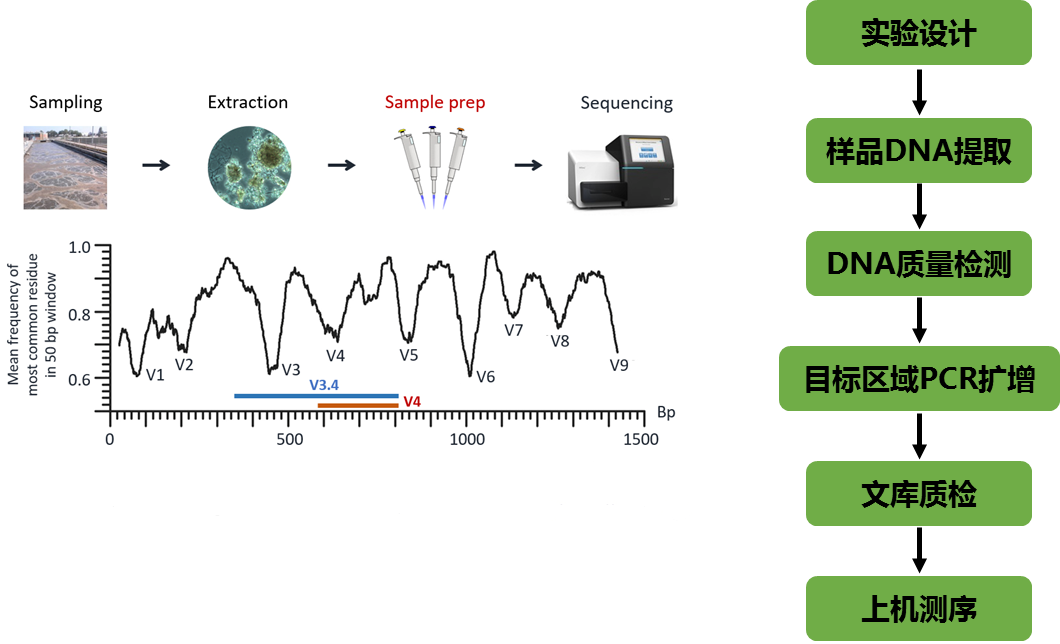
\includegraphics[width=0.8\textwidth]{./figures/theme/16s_实验流程.png}  
\end{figure}
%%%%%%%%%%%%%%%%%%%%%%%%%%%%%%%%%%%%%%%%%%%%%%%%%%%%%%%
\newpage
\subsection{生物信息分析流程}
\label{Subsec:bioinformaticAnalyzeFlow}
\begin{figure}[H]
\centering
\label{Fig:bioinformaticAnalyzeFlow111}
 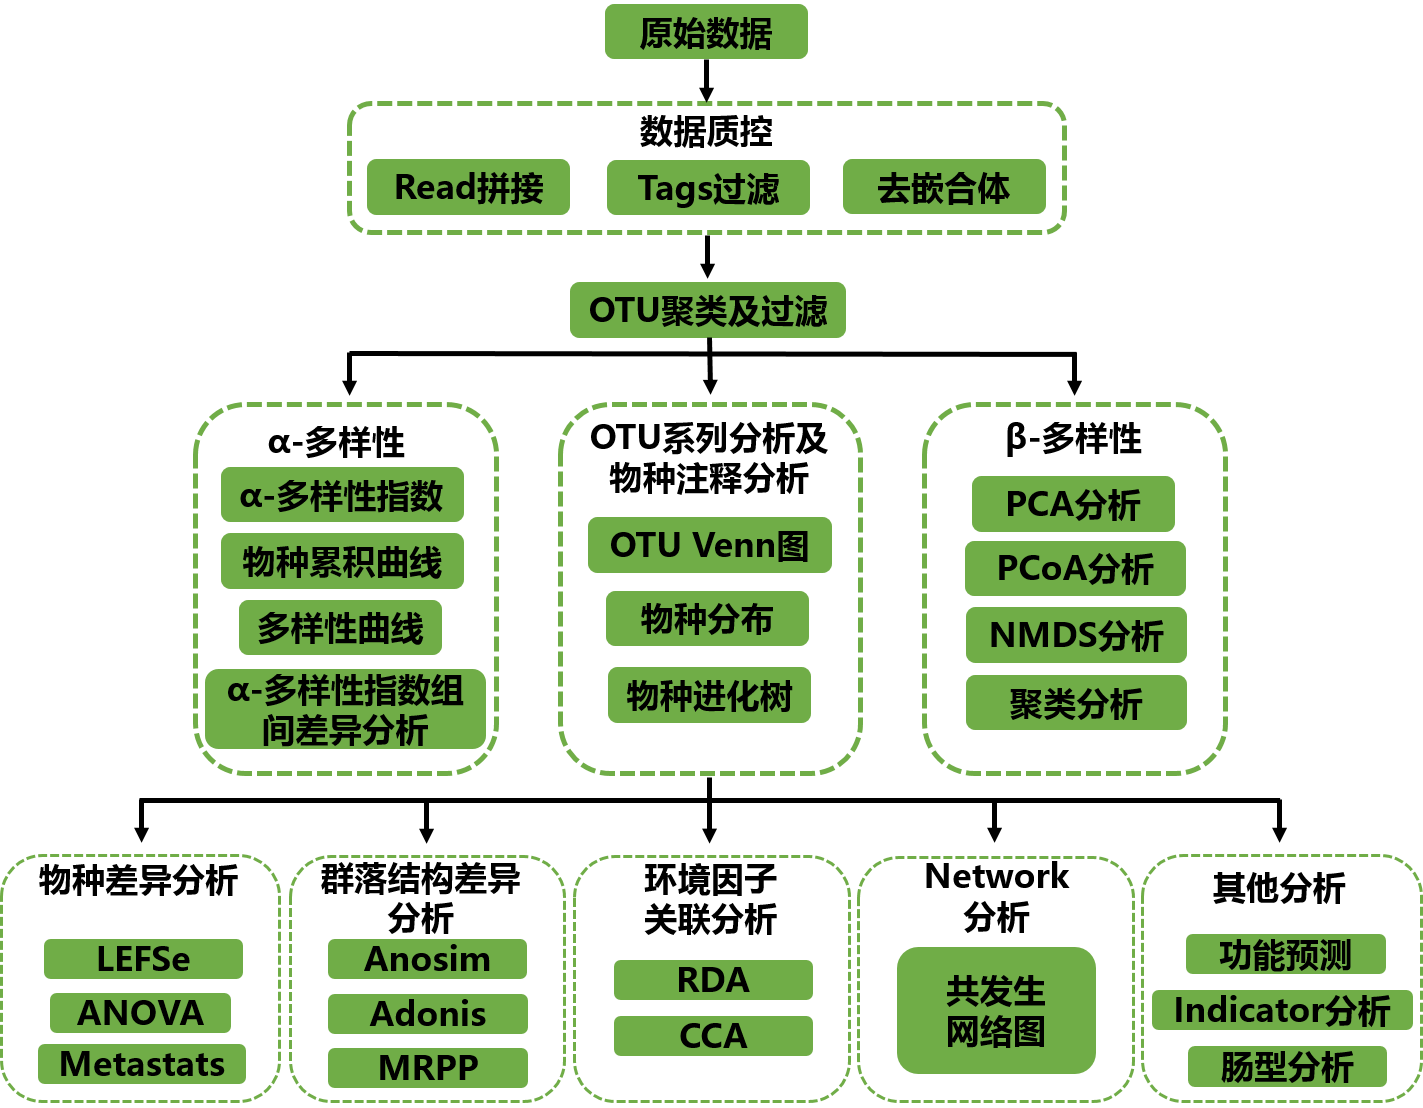
\includegraphics[width=0.8\textwidth]{./figures/theme/16s_生物信息分析流程素材.png}  
\end{figure}
\begin{table}[H]
\renewcommand\arraystretch{1.0}
\begin{tabular}{|p{.14\textwidth}<{\centering}|p{.14\textwidth}<{\centering}|p{.3\textwidth}<{\centering}|p{.32\textwidth}<{\centering}|}
\rowcolor{anjieGreen}
\hline
\textbf{基本分析}&\textbf{标准分析}&\textbf{高级分析}&\textbf{个性化分析}\\
\hline
序列拼接、质控&物种分布图&LEFSe 分析&\multirow{1}{*}{物种间相关性分析}\\
\cline{1-3}
OTU 聚类&Shannon 指数& Anosim 分析(组内大于 5 个重复)&(需提供相关物种)\\
\hline
物种注释& Chao 指数& ANOVA 分析(组内大于 3 个重复)&\multirow{1}{*}{物种与环境相关性分析  }\\
\cline{1-3}
稀释曲线& Simpson 指数& RDA 分析(需提供环境因子)&(需提供相关物种与环境因子)\\
\hline
Shannon 曲线&PCA 分析& CCA 分析(需提供环境因子) &客户定制化分析\\
\hline
\multirow{2}{*}{Simpson 曲线}&PCoA 分析 &物种分类树& 客户定制化绘图\\
\cline{2-4} 
&Heatmap 图 &功能预测分析&\\
\hline
\end{tabular}
\end{table}

%%%%%%%%%%%%%%%%%%%%%%%%%%%%%%%%%%%%%%%%%%%%%%%%%%%%%
\newpage
\section{分析内容}
\label{Sec:Maincontent}
\subsection{原始数据质控}
\label{Subsec:RawDataQualityContral}
测序原始数据以FASTQ格式保存,每条read 包含4行信息:第一行以“$@$”起始,包含序列ID和相应的描述信息;第二行为碱基序列,其中N表示模糊碱基;第三行为“+”;第四行代表reads对应碱基的测序质量。\\
{$@$HISEQ15:146:C6VAJANXX:7:1101:6695:1978 1:N:0:TCATTC\\
ATCGGAAGAGCACACGTCTGAACTCCAGTCACTCATTCATCTCGTATGCCGTCTT\\
+\\
=<ABFGGGGGGGGGGGEGEFGGGGGGDGEFGG@GGFFGGF1BFFEFEGGGGGGG}

原始数据存在低质量、可能的接头等序列,为了确保分析结果的可靠准确,需要先将这部分序列去除才能用于下一步的分析。

% \begin{table}[H]
% \centering
% \caption{ 数据质控统计}
%  \footnotesize
%  \label{table:RawDataQualityContral}
%  \begin{tabular}{p{.10\textwidth}<{\centering} p{.14\textwidth}<{\centering} p{.12\textwidth}<{\centering} p{.12\textwidth}<{\centering}p{.12\textwidth}<{\centering}p{.1\textwidth}<{\centering}p{.14\textwidth}<{\centering} }
%   \toprule
%   Sample&ReadLength(bp)&InterSize(bp)&RawData&CleanData&UseRate(\%)&GC(\%) \\
%   \midrule
%  Sample 1& 150 & 510&380,848,928&329,966,668&86.64&63\\
%  Sample 2& 150 & 523&364,312,762&320,047,870&87.85&61\\
%  Sample 3& 150 & 514&364,644,846&315,124,066&86.42&62\\
%   \bottomrule
%  \end{tabular}
% \end{table}

\begin{figure}[H]
\centering 
\captionsetup{width=.7\textwidth,singlelinecheck = false, justification=justified}
\label{Fig:Position_In_Reads}
 \includegraphics[width=0.7\textwidth]{./figures/1_clean_reads/1_1_base_quality/HBT-12_clean_merge.png}  
 \caption{Reads各位置碱基质量分布。横坐标为reads 碱基坐标,纵坐标为碱基质量值,蓝色线代表平均质量值。横轴表示测序的碱基排序位置,纵轴表示该位置上碱基的平均质量,用 Phred quality
score 表示,质量为 20 表示该位置的碱基准确度达到 99\%,该图为拼接的 reads 质量分布,因为采用双端测序,拼接后质量较差的集中在中间部位。}
\end{figure}
%%%%%%%%%%%%%%%%%%%%%%%%%%%%%%%%%%%%%%%%%%%%%%%%%%%%%%%%
\newpage
\subsection{OTU 结果统计及稀释曲线分析}
\label{Subsec:OTUAnnotation}
\subsubsection{拼接序列统计}
\label{Subsubsec:seqanalysis}
采用Illumina Hiseq测序平台得到的下机双端数据,我们称之为原始数据(Raw reads),采用Flash软件 \cite{Mago2011FLASH} 进行拼接和质控得到高质量的Clean\ reads,再进行嵌合体过滤(Chimera\_check),最后采用QIIME软件\cite{Caporaso2010QIIME}进行OTU聚类,获得各样品的OTU丰度表格。各步骤的数据统计见表3.1。
\begin{table}[H]
\begin{threeparttable}
\captionsetup{singlelinecheck = true}
 \caption{拼接序列统计}
 \label{table:seqanalysis}
 \footnotesize
 \begin{tabular}{p{.14\textwidth}<{\centering} p{.14\textwidth}<{\centering} p{.14\textwidth}<{\centering} p{.14\textwidth}<{\centering}p{.14\textwidth}<{\centering}p{.14\textwidth}<{\centering}}
 \toprule
 Sample&Raw&Clean&Chimera\_check&OTUseq&OTU\\
  \midrule
HBT-12&210925&170032&158387&156758&315\\
HBT-8&183083&158345&144111&142813&300\\
HBV-11&146406&123711&107866&105611&224\\
HBV-12&111857&94888&84164&83528&222\\
HBV-22&147494&109328&100453&100086&259\\
HBV-46&137829&120541&109743&109039&235\\
HBV-5&136264&117697&107035&105830&198\\
HBV-52&223078&186910&168071&167289&375\\
HBV-56&160007&142483&126229&125695&185\\
HBV-59&131681&113029&97809&97074&121\\
HBV-61&178263&153457&136858&135428&375\\
HBV-64&160438&139820&125382&124550&269\\
HBV-68&166270&145708&131593&120095&256\\
IMT17&264255&225437&198634&197823&264\\
N39&337918&280695&247820&245104&307\\
N41&182956&134404&125245&124217&335\\
N42&148842&109498&102180&101888&234\\
N43&150334&95425&87564&87009&289\\
N44&157824&127092&118789&118049&316\\
  \bottomrule
 \end{tabular}
 \begin{tablenotes}
 \footnotesize
\item[1] Raw 为原始测序的 reads 数,Clean 表示每个样品质控后的 reads 数,所用拼
接软件为 Flash;Chimera\_check 表示去除嵌合体后的序列数;OTUseq 为具有 OTU 从
属的序列数,OTU 为每个样本聚类得到的 OTU 数。
\item[2] 表格详见文件夹 report/2\_OTU\_assembly\_analysis/2\_2\_assemble\_table/下的.xls
文件。
\end{tablenotes}
\end{threeparttable}
\end{table}
%%%%%%%%%%%%%%%%%%%%%%%%%%%%%%%%%%%%
\newpage
\subsubsection{Rarefaction 稀释曲线}
\label{Subsubsec:rarefactionCurvy}
对每个样品的测序序列进行随机抽样方法,以抽到的序列数与它们能代表的数目构建曲线,即稀释曲线。当曲线趋于平坦时,说明测序数据量合理,更多的数据量对于发现新的OTU的贡献很小;反之则表明测序不足,继续测序可能可以产生新的物种,由Qiime \cite{Caporaso2010QIIME} 分析得到。
\begin{figure}[H]
\captionsetup{width=.8\textwidth,singlelinecheck = false, justification=justified}
\centering
\label{Fig:rarefactionCurvy}
 \includegraphics[width=0.8\textwidth]{./figures/theme/RarefactionCurve.png}  
 \caption{稀释曲线图(Rarefaction Curve)。横轴表示随机抽取的序列数,纵轴表示对应的可以检测到的OTU数。}
\end{figure}
%%%%%%%%%%%%%%%%%%%%%%%%%%%%%%%%%%%%%%%%%%%%%%%%%%%%%%

\newpage
\subsubsection{Shannon-Wiener曲线}
\label{Subsubsec:Shannon-Wiener}
Shannon-Wiener指数是反映样品中微生物多样性的指数。Shannon-Wiener曲线利用各样品的测序量在不同测序深度时的Shannon-Wiener指数构建曲线,以此反映各样本在不同测序数量时的微生物多样性。 
\begin{figure}[H]
\captionsetup{width=.8\textwidth,singlelinecheck = false, justification=justified}
\centering
\label{Fig:shannnon-wiener}
 \includegraphics[width=0.8\textwidth]{./figures/theme/Shannon-Wiener曲线.png}  
 \caption{Shannon-Wiener曲线。 横轴表示样品中不同的测序深度,纵轴表示对应深度下的Shannon-Wiener指数,不同的颜色的曲线代表不同样品的Shannon-Wiener曲线,曲线升高直至平滑说明测序深度足够可以覆盖样品中的大部分微生物。}
\end{figure}

Shannon-wiener指数计算公式为:
\begin{equation*}
\centering
 \mathrm{\textbf{H}}_{\mathrm{Shannon}}=-\sum^{\mathrm{S}_{\mathrm{obs}}}_{i=1}\frac{n_i}{N}\ln{\frac{n_i}{N}}\mathrm{,}
\end{equation*}
其中,
$\rm{S}_{\rm{obs}}$为实际测量出的OTU数目;
$n_{i}$为含有$i$条序列的OTU数目;
$N$为所有序列数。

%%%%%%%%%%%%%%%%%%%%%%%%%%%%%%%%%


\newpage
\subsubsection{Simpson稀释曲线}
\label{Subsubsec:Simpson稀释曲线}
Simpson稀释曲线,是利用各个样品在不同测序量下的Simpson多样性指数构建曲线的,以此也可以反映各个样品在不同测序深度下的微生物多样性。
\begin{figure}[H]
\captionsetup{width=.8\textwidth,singlelinecheck = false, justification=justified}
\centering
\label{Fig:Simpson稀释曲线}
 \includegraphics[width=0.8\textwidth]{./figures/theme/Simpson稀释曲线}  
 \caption{Simpson稀释曲线。 横轴表示样品中不同的测序深度,纵轴表示对应深度下的Simpson指数,不同的颜色的曲线代表不同样品的Simpson曲线,曲线升高直至平滑说明测序深度足够可以覆盖样品中的大部分微生物。}
\end{figure}

Simpson指数计算公式为:
\begin{equation*}
\centering
 \mathrm{\textbf{D}}_{\mathrm{simpson}}=\frac{\sum^{\mathrm{S}_{\mathrm{obs}}}_{i=1}n_i(n_i-1)}{N(N-1)} \mathrm{,}
\end{equation*}
其中,
$\rm{S}_{\rm{obs}}$为实际测量出的OTU数目;
$n_{i}$为含有$i$条序列的OTU数目;
$N$为所有序列数。

%%%%%%%%%%%%%%%%%%%%%%%%%%%%%%%%%
\newpage
\subsubsection{样品OTU分布Venn图}
\label{Subsubsec:OTU-Venn}
用来统计多个样品中共有或独有的OTU数目,可以比较直观地反映出环境样品之间的OTU组成相似程度。注:所提供样本分组至少两个,最多5个。
\begin{figure}[H]
\centering
\label{Fig:OTU——venn}
\captionsetup{width=.8\textwidth,singlelinecheck = false, justification=justified}
 \includegraphics[width=0.8\textwidth]{./figures/theme/样品OTU分布Venn图.png}  
  \caption{不同颜色代表不同的组样本,中间数字代表每个色块的OTU数目,色块的重叠区代表共有OTU。}
\end{figure}


%%%%%%%%%%%%%%%%%%%%%%%%%%%%%%%%%%%%%%%%%%%%%%%%%%%%%%%%%%%%%%%%%

\newpage

\subsection{样本物种组成成分分析}
\label{Subsec: Component Analysis}
根据物种分类结果,可以统计出每个样品在各个分类水平上的物种组成比例,反映样品在不同分类学水平的群落结构。
\begin{figure}[H]
\centering
\label{Fig:样本菌群结构聚类图}
\captionsetup{width=.8\textwidth,singlelinecheck = false, justification=justified}
 \includegraphics[width=0.8\textwidth]{./figures/theme/样本菌群结构.png}  
   \caption{样本菌群结构。分样本在门、纲、目、科、属、种水平的前30种优势物种的结构菌群结构柱状图,不同微生物物种用不同颜色表示,横轴表示样品编号,纵轴表示物种相对丰度。}
\end{figure}

%%%%%%%%%%%%%%%%%%%%%%%%%%%%%%%%%%%%%%%%%%%%%%%%%%%%%%
\newpage

\subsection{$\alpha$多样性分析}

$\alpha$多样性分析用于分析样品内微生物群落组成的复杂程度。通过单样本的$\alpha$多样性指数,可以反映样品内的微生物群落的丰富度(ACE、Chao1、Observed species)、多样性(Shannon和Simpson)以及均匀度(J)。

%\begin{table}[H]
%\begin{threeparttable}
%\captionsetup{singlelinecheck = true}
% \caption{拼接序列统计}
% \label{table: Alphadiverstiy}
% \footnotesize
%  \begin{tabular}{p{.11\textwidth}<{\centering} p{.11\textwidth}<{\centering}p{.11\textwidth}<{\centering} p{.12\textwidth}<{\centering} p{.14\textwidth}<{\centering}p{.12\textwidth}<{\centering}p{.12\textwidth}<{\centering}}
% \toprule
% Sample&ACE&Chao1&Shannon&Observed\_species&Goods\_coverage&Simpson\\
%  \midrule
%JC01&2690.49397544&2673.06666667&7.01443000676&	2056.0&0.993834296724&0.967667979485\\
%JC02&2601.78895713&2525.97183099&7.0380870341&1859.0&0.992826031258&0.965952343561\\
%JC03&2490.95661567&2425.85393258&7.29933587517&1764.0&0.992035872039&0.979466364755\\
%JC04&2681.42716543&2644.54416961&7.66260462799&1922.0&0.990482280683&0.985153804737\\
%JC05&2646.33759745&2548.00961538&7.23296008947&1929.0&0.99301319854&0.979110069467\\
%JC06&2401.09224937&2370.34108527&6.75657500898&1744.0&0.992724064294&0.958643124067\\
%JC07&2710.64544094&2668.78595318&7.33618552114&1959.0&0.99154980689&0.977492246003\\
%JC08&2883.16090298&2869.38032787&7.27393505664&2108.0&0.992586473031&0.977125735307\\
% \bottomrule
% \end{tabular}
% \begin{tablenotes}
% \footnotesize
%\item[1] 表格详见文件夹report/ 3alpha\_diversity下的.xls文件。
%\end{tablenotes}
%\end{threeparttable}
%\end{table}
%%%%%%%%%%%%%%%%%%%%%%%%%%%%%%%%%%%%%%%%%%%%%%%%%%%%%%%
\begin{figure}[H]
 \centering
\captionsetup{width=.8\textwidth,singlelinecheck=false,justification=justified}
\label{Fig:diversity}
\captionsetup{width=.8\textwidth,singlelinecheck=false,justification=justified}
 \includegraphics[width=0.8\textwidth]{./figures/theme/alpha_diversity_boxplot.png}
    \caption{Alpha多样性指数箱型图。横坐标表示样品分组,纵坐标为alpha指数,表格详见文件夹report/group*/ 4alpha\_diversity下的.xls文件}
\end{figure}


%%%%%%%%%%%%%%%%%%%%%%%%%%%%%%%%%%%%%%%%%%%%%%%%%%%%%%%%
\newpage

\subsection{ANOSIM相似性分析}
\label{Subsec: ANOSIM}
相似性分析Analysis of similarities(ANOSIM)是一种非参数检验,用来检验组间(两组或多组)的差异是否显著大于组内差异,从而判断分组是否有意义。首先利用Bray-Curtis算法计算两两样品间的距离,然后将所有距离从小到大进行排序。
\begin{figure}[H]
\centering
\captionsetup{width=.8\textwidth,singlelinecheck = false, justification=justified}
\label{Fig:ANOSIM}
\captionsetup{width=.8\textwidth,singlelinecheck = false, justification=justified}
 \includegraphics[width=0.8\textwidth]{./figures/theme/ANOSIM.png}  
   \caption{ANOSIM。横坐标表示所有样品(Between)以及每个分组,纵坐标表示距离的秩。Between组比其它每个分组的秩较高时,则表明组间差异大于组内差异。R$\in$(-1,1)之间,R>0,说明组间差异显著;R<0,说明组内差异大于组间差异,若两个分组的凹槽互不重叠,则表明它们的中位数有显著差异,统计分析的可信度用P表示,P< 0.05表示统计具有显著性。}
\end{figure}

%%%%%%%%%%%%%%%%%%%%%%%%%%%%%%%%%%%%%%%%%%%%%%%%%%%%%%
\newpage

\subsection{$\beta$多样性分析}
\label{Subsec: betaadiverstiy}
$\beta$ Diversity是对不同样品的微生物群落结构进行比较分析。由于每个样品含有大量的OTU种类(维度),因此通常采用多变量统计学方法对数据进行降维处理,以直观展示样品间的差异。常用的降维方法包括主成分分析(PCA,Principal Component Analysis)、主坐标分析(PCoA,Principal Co-ordinates Analysis)和非度量多维尺度分析(NMDS,Non-Metric Multi-Dimensional Scaling)。其中,PCA基于各样品的OTU丰度数据进行,而PCoA和NMDS基于UniFrac距离(同时考虑OTU丰度和OTU之间的遗传距离的大小)进行。
\subsubsection{PCA分析}
\label{Subsubsec:PCA}
PCA是一种简化数据集的技术,可以去除数据噪音和冗余,将原有的复杂数据降维,从而揭示隐藏在复杂数据背后的简单结构。它可以在减少数据集的维数的情况下,同时保持数据集中对方差贡献差异最大的特征,从而有效地找出数据中最主要元素。
\begin{figure}[H]
\centering
\label{Fig:PCA}
\captionsetup{width=.8\textwidth,singlelinecheck = false, justification=justified}
 \includegraphics[width=0.8\textwidth]{./figures/theme/pca分析.png}  
   \caption{PCA分析结果散点图。 图中每个点为一个样本,不同颜色表示不同实验设计的组别,点与点的距离越近,表明样本越相似。PCA是利用样品的物种丰度矩阵所做的排序分析,横轴与纵轴表示的分别是第一主成分(PC1)和第二主成分(PC2)的贡献率。}
\end{figure}
%%%%%%%%%%%%%%%%%%%%%%%%%%%%%%%%%%%%%%%%%%%%%%%%%%%%%%
\newpage
\subsubsection{PCoA分析}
\label{Subsubsec:PCoA}
PCoA是一种研究数据相似性与差异性的方法,与PCA分析的区别是PCA分析只是基于原始的物种组成矩阵所做的排序分析,而PCoA分析则是基于物种组成计算得到的距离矩阵得出的。在PCoA分析中,计算距离矩阵的方法有很多,UniFracs,Euclidean, Bray-Curtis与Jaccard,默认情况选择UniFracs,所用的R包为Phyloseq \cite{Mcmurdie2013phyloseq}。
\begin{figure}[H]
\centering
\label{Fig:PCOA}
\captionsetup{width=.8\textwidth,singlelinecheck = false, justification=justified}
 \includegraphics[width=0.8\textwidth]{./figures/theme/pcoa分析.png}  
   \caption{PCoA分析结果散点图。 图中每个点为一个样本,不同颜色表示不同实验设计的组别,点与点的距离越近,表明样本越相似.PCoA是利用样品的物种组成计算得到的距离矩阵进行分析的,横轴与纵轴表示的分别是第一主成分(PC1)和第二主成分2(PC2)的贡献率。}
\end{figure}
%%%%%%%%%%%%%%%%%%%%%%%%%%%%%%%%%%%%%%%%%%%%%%%%%%%%%%%
\newpage
\subsubsection{NMDS分析}
\label{Subsubsec:NMDS}
NMDS是一种基于样本距离矩阵的MDS分析方法,通过降维处理简化数据结构,在新的低维坐标系中对样本重新排序,从而在特定距离尺度下描述样本的分布特征。与PCoA分析不同,NMDS分析不依赖于特征值和特征向量的计算,而是通过对样本距离进行等级排序,使样本在低维空间中的排序尽可能符合彼此之间的距离远近关系(而非确切的距离数值)。因此,NMDS分析不受样本距离的数值影响,仅考虑彼此之间的大小关系,对于结构复杂的数据,排序结果可能更稳定。
\begin{figure}[H]
\centering
\label{Fig:NMDS}
\captionsetup{width=.8\textwidth,singlelinecheck = false, justification=justified}
 \includegraphics[width=0.8\textwidth]{./figures/theme/nmds分析.png}  
   \caption{NMDS分析结果散点图。 每一个点代表一个样本,相同颜色的点来自同一个分组,两点间的距离越近表明两者的群落结构差异越小。}
\end{figure}
%%%%%%%%%%%%%%%%%%%%%%%%%%%%%%%%%%%%%%%%%%%%%%%%%%%%%%
\newpage
\subsection{样本及物种聚类分析}
\label{Subsec: clustering}
\subsubsection{样本及物种聚类热图}
\label{Subsubsec:clusteringheatmap}
根据OTU数据进行标准化后,选取数目最多的前30个物种,然后进行作图。热图中的物种聚类距离默认选择correlation方法,样本聚类距离默认选择Bray-Curtis方法。热图中的每一个色块表示一个样品的一个分类水平的丰度。样本聚类热图可以提供样品之间的相似性以及差异性信息,还有对应分类水平的群落构成相似性。
\begin{figure}[H]
\centering
\label{Fig:clusteringHeatMap}
\captionsetup{width=.8\textwidth,singlelinecheck = false, justification=justified}
 \includegraphics[width=0.8\textwidth]{./figures/theme/heatmap_f.png}  
   \caption{样本及物种聚类热图。 在不同分类水平的样本间前30种优势物种在样本间的聚类, 不同颜色表示不同的物种丰度比例。物种间的相似关系和样本间的相似关系分别表示在图片的左方和上方。}
\end{figure}

%%%%%%%%%%%%%%%%%%%%%%%%%%%%%%%%%%%%%%%%%%%%%%%%%%%%%%
\newpage
\subsubsection{样本无聚类热图}
\label{Subsubsec:non-clusteringheatmap}
同\ref{Subsubsec:clusteringheatmap},只是不展示样本间的聚类图。
\begin{figure}[H]
\centering
\label{Fig:clusteringheatmapnoclust}
\captionsetup{width=.8\textwidth,singlelinecheck = false, justification=justified}
 \includegraphics[width=0.8\textwidth]{./figures/theme/heatmap_f_noclust.png}  
   \caption{与图 3.12 类似,样本间前30种优势物种在样本间的热图, 不同颜色表示不同的物种丰度比例,样本间的相似关系分别表示在图片的左方, 但是没有展示样本间的相似关系。}
\end{figure}

%\ref{Fig:clusteringHeatMap}
%%%%%%%%%%%%%%%%%%%%%%%%%%%%%%%%%%%%%%%%
\newpage
\subsubsection{样本菌群结构聚类}
\label{Subsubsec:biota}
根据样品在不同分类水平下的丰度进行聚类,并绘制对应样本树状图对应样本的群落结构。

\begin{figure}[H]
\centering
\label{Fig:clusteringbiota}
\captionsetup{width=.8\textwidth,singlelinecheck = false, justification=justified}
 \includegraphics[width=0.8\textwidth]{./figures/theme/样本菌群结构聚类.png}  
   \caption{样本菌群结构聚类图。 利用所有的物种信息在不同分类水平构建的样本聚类结果图,右边为该分类水平下的菌群结构}
\end{figure}
%%%%%%%%%%%%%%%%%%%%%%%%%%%%%%%%%%%%%%%%
\newpage
\subsubsection{样本无菌群结构聚类}
\label{Subsubsec:clusteringnobiota}
根据样品在门、纲、目、科、属等不同分类水平下的丰度进行分析,绘制样本在相应分类水平下的聚类树状图,但不展示对样本中菌群结构组成。

\begin{figure}[H]
\centering
\label{Fig:clusteringnobiota}
\captionsetup{width=.8\textwidth,singlelinecheck = false, justification=justified}
 \includegraphics[width=0.8\textwidth]{./figures/theme/genus_cluster.png}  
   \caption{样本无菌群结构聚类图。 与图 3.14 类似,利用所有的物种信息在不同分类水平构建的样本聚类结果图,但是没有相应的菌群结构。}
\end{figure}
 %\ref{Fig:clusteringbiota}
%%%%%%%%%%%%%%%%%%%%%%%%%%%%%%%%%%%%%%%%
\newpage
\subsection{样本菌群总览图}
\label{Subsec: allBioinSample}
将不同组的样本群落构成以及分布以物种分类树的形式展示在一个环形图中。数据经过分析后,将物种分类树与分类丰度信息通过软件 GraPhlAn \cite{Asnicar2015Compact} 进行绘制的。可以展示物种之间的进化关系以及不同样本的物种分布丰度和最高分布样本。
\begin{figure}[H]
\centering
\label{Fig:allBioinSample}
\captionsetup{width=.8\textwidth,singlelinecheck = false, justification=justified}
 \includegraphics[width=0.8\textwidth]{./figures/theme/样本菌群总览图.png}  
   \caption{样本菌群总览图。图中间的圈图为物种进化分析,不同颜色分子代表了不同门分类水平(由右上角的颜
色标注);灰色标注的是丰度前 15 个科(A-O)的分布情况。次外圈的热图表示不同组的物种(组
名在圈内 6 点钟方向),用不同的颜色表示不同的组,颜色深浅表示相应物种的丰度。最外圈为
相应的物种在不同组的最大丰度,颜色用具有最大丰度的组的颜色表示。}
\end{figure}


%%%%%%%%%%%%%%%%%%%%%%%%%%%%%%%%%%%%%%%%
\newpage
\subsection{物种差异分析}
\label{Subsec:speciesDiff}
LEfSe \cite{Paulson2013Differential} 分析即 LDA Effect Size 分析,可以实现多个分组之间的比较,同时进行分组比较的内部进行亚组比较分析,从而找到组间在丰度上有显著差异的物种。其主要原理如下:

(1)首先在多组样本中采用非参数因子 、 Kruskal-Wallis秩和检验方法检测不同分组之间丰度差异显著的物种; 
(2)对上一步差异显著物种,用成组的 Wilcoxon 秩和检验来分析组间差异;
(3)最终用线性判别分析 Linear Discriminant Analysis (LDA)对数据进行降维和评估差异显著的物种的影响力(即 LDA score)。

\begin{figure}[H]
\centering
\label{Fig:LEfSe}
\captionsetup{width=.8\textwidth,singlelinecheck = false, justification=justified}
 \includegraphics[width=0.8\textwidth]{./figures/theme/LEfSe分析.png}
 \caption{LDA 值分布圈图,展示的是 LDA Score 大于设定值有差异的物种,即具有统计
学差异的 biomaker。 同时展示不同组中丰度具有显著差异的物种,柱状图的长度表示显著
差异物种的影响大小。}
\end{figure}

\begin{figure}[H]
\centering
\label{Fig:LEfSe2}
\captionsetup{width=.8\textwidth,singlelinecheck = false, justification=justified}
 \includegraphics[width=0.8\textwidth]{./figures/theme/LEfSe分析2.png}
 \caption{进化关系图,由内到外辐射的圆圈代表了由门至属(或种)的分类级别。在不同分类级别上的每个小圆圈代表该水平下的一个分类,小圆圈直径大小与相对丰度大小呈正比。其中无显著差异的物种为黄色,差异物种则与跟随组别进行着色。右上角为对应的圈图内英文字母的物种名称。}
\end{figure}

\begin{figure}[H]
\centering
\label{Fig:LEfSe3}
\captionsetup{width=.8\textwidth,singlelinecheck = false, justification=justified}
 \includegraphics[width=0.8\textwidth]{./figures/theme/LEfSe分析3.png}
 \caption{biomaker在不同组内各样本中的丰度比较图.将丰度最高的biomaker的样本的丰度设定为1,其他样品中该biomaker的丰度为相对丰度最高样品的相对值。}
\end{figure}

%%%%%%%%%%%%%%%%%%%%%%%%%%%%%%%%%%%%%%%%%%%%%%%%%%%%%%
\newpage
\subsection{功能分析}
\label{Subsec: functionalAnalysis}
通过 16s 测序数据获得了样本中的物种信息,结合已经测得的宏基因组基
因功能的构成数据进行功能预测,然后可以对不同样品和分组之间在功能上的差
异进行分析等。主要利用的是 PICRUSt \cite{Langille2013Predictive}软件。该软件基本原理是通过 16s 测
序数据与已知的宏基因组的功能数据比较分析,然后推测 16s 样本的功能。此
方法在肠道微生物与土壤菌群的功能分析接近 95\%,可以很好的反映出样品中
的功能基因构成。我们提供 COG 以及 KEGG 代谢通路途径分析 \cite{Kanehisa2008KEGG}。
\subsubsection{KEGG 代谢通路分析}
\label{Subsubsec:KEGG}
通过 KEGG 代谢途径的预测不同组间的差异分析,可以了解到组间微生物
群落的功能基因在代谢途径上的差异。
\begin{figure}[H]
\centering
\label{Fig:kegg}
\captionsetup{width=.8\textwidth,singlelinecheck = false, justification=justified}
 \includegraphics[width=0.8\textwidth]{./figures/theme/kegg.png}  
   \caption{KEGG代谢通路分析图。 图左表示差异显著的 kegg 通路在组间(不同颜色)的分布,柱长表示对应样本
在该代谢通路中功能基因的丰度,error bar 表示丰度标准误的大小;图右表示方差分析
检验的 P 值的大小,颜色值越大表示不同组间的差异越显著。}
\end{figure}
%%%%%%%%%%%%%%%%%%%%%%%%%%%%%%%%%%%%%%%%
\newpage

\subsubsection{COG 分析}
\label{Subsubsec:COG}
利用 PICRUSt 预测到的样本的 COG 注释信息,分析组间 COG 功能分类的差异。
\begin{figure}[H]
\centering
\label{Fig:COG}
\captionsetup{width=.8\textwidth,singlelinecheck = false, justification=justified}
 \includegraphics[width=0.8\textwidth]{./figures/theme/cog.png}  
   \caption{COG分析图。 图左表示差异显著的 COG 功能在组间(不同颜色)的分布,柱长表示对应样本
在该代谢通路中功能基因的丰度,error bar 表示丰度标准误的大小;图右表示方差分析检
验的 P 值的大小,颜色值表示不同组间的差异越显著。}
\end{figure}
%%%%%%%%%%%%%%%%%%%%%%%%%%%%%%%%%%%%%%%%
%\newpage
%\subsection{高级分析}
%\subsubsection{indicator taxa 分析}
%indicator taxa 分析是一种计算任何分类群在不同分组中被发现的可能性的方法,以及在给定的分组之外发现同一个分类群的概率,
%我们使用indicspecies\cite{indicspecies}软件包计算分类群在不同分组种的指标值(IndVal),并进行统计学检验。当指标值(IndVal)越高时,
%表明该分类群在给定的分组中出现的概率越大,也是一种查找差异物种的常用分析方法。
%\begin{figure}
% \label{FIG:indicator}
%\centering
% \captionsetup{width=.8\textwidth,singlelinecheck = false, justification=justified}
%\includegraphics[width=0.8\textwidth]{./figures/theme/indicator_bar_plot.png}
%\caption{indicator 概率图。左边的柱状图是具有显著性差异的物种在所有样品中的平均相对丰度,不同颜色代表不同的门水平在左边图例展示,
%右边是不同分组中对应物种在该组中的指示值(IndVal),圆圈越大代表该物种在该分组中出现的可能性越大,不同颜色代表不同分组。 }
% \end{figure}





%%%%%%%%%%%%%%%%%%%%%%%%%%%%%%%%%%%%%%%%%%%%%
\newpage
\section*{附录:文件结构}\sectionmark{附录:文件结构}
%\setcounter{section}{4}
\addcontentsline{toc}{section}{附录:文件结构}
\footnotesize
    \dirtree{%
.1 /.
.2 0\_raw\_reads.
.3 0\_1\_base\_quality|…*\_quality.png                      [原始reads质量分布图].                               
.2 1\_clean\_reads.
.3 1\_1\_base\_quality|…*\_quality.png                  [拼接过滤后序列质量分布图].
.2 2\_OTU\_assembly\_analysis.
.3 2\_1\_species\_distribution│…*.svg;*xls[不同分类水平下在样本中分布柱状图以及表格].
.3 2\_2\_assemble\_table│sample2sequence\_summary.xls [reads以及otu统计汇总表].
%.3 2\_2\_assemble\_table│otus.fa [otu代表序列].
%.3 2\_2\_assemble\_table│*.tre [进化树表格].
%.3 ……otu\_table\_norm.xls                                  [标准化后的otu丰度表格].
.3 ……otu\_tax\_table\_norm.xls             [标准化后的otu丰度表格,含有物种注释信息].
.3 ……otu\_tax\_table.xls                  [未标准化的otu丰度表格,含有物种注释信息].
%.3 ……otu\_tax\_table\_norm.biom               [标准化后的otu丰度表格,为biom格式].
%.3 ……otu\_tax\_table.biom                     [未标准化的otu丰度表格,为biom格式].
%.3 ……multi\_adiversity.xls                           [各样品的物种多样性指数汇总表].
%.3 ……richness\_plot.svg                           [不同分析的相关物种多样性盒形图].
.2 3\_rarefaction.
.3 …… *.svg                                           [各样品的多样性指数曲线图].
.2 group*.
.3 5\_Anosim\_analysis.
.4 ……anosim\_plot.svg|otu\_table\_norm.xls                                  [Anosim相似性分析盒形图以及相似性统计数据].
.3 6\_beta\_diversity.
.4 6\_1\_ordinatioin│……pca\_plot.svg                          [PCA分析结果图].
.4 6\_1\_ordinatioin│……PCoA\_plot.svg                       [PCoA分析结果图].
.4 6\_1\_ordinatioin│……NMDS\_plot.svg                      [NMDS分析结果图].
.4 6\_2\_heatmap.
.5 6\_2\_1\_with\_clust│…*.svg    [有样本聚类信息的各个分类水平的heatmap图].
.5 6\_2\_2\_without\_clust│…*.svg   [没有样本聚类的各个分类水平的heatmap图].
.5 ……*.xls                                        [为heatmap分析的输入统计数据].
.4 6\_3\_clust│…*.svg;*xls      [为物种组成结构及样本聚类图以及相应的输入数据].
.3 7\_environment\_factor.
.4 7\_1\_CCA│……cca\_plot.svg               [CCA分析结果图(需提供环境因子)].
.4 7\_2\_RDA│……rda\_plot.svg                [RDA分析结果图(需提供环境因子)].
.3 8\_species\_visulization.
.4 speciese\_distribution\_group.svg    [物种分类进化树以及样品组间差异情况总览图].
.3 9\_differential\_species\_analysis.
.4 9\_1\_LEFSe\_analysis.
.5 ……otu\_table\_lefse\_LDA.svg                [LEFSe差异分析的LDA柱状图].
.5 ……otu\_table\_lefse\_cladogram.svg                 [LEFSe差异物种树形图].
.5 differential\_species\_distribution            [LEFSe分析的差异物种柱状图].
.3 10\_function\_analysis.
.4 10\_1\_KEGG│……KEGG\_pathway.svg         [KEGG通路预测结果差异分析图].
.4 10\_1\_KEGG│……kegg\_pathway\_prediction\_count.xls     [KEGG预测结果总表].
.4 10\_2\_COG│……COG\_function.svg             [COG功能预测结果差异分析图].
.4 10\_2\_COG│……cog\_prediction\_count.xls                 [COG预测结果总表].
.4 ……picrust\_otus\_css.biom                   [功能预测软件PICRUSt预测结果文件].
    }
注:生物信息分析相关文件均在Linux系统下产生。在Windows在的文本文件一般用写字板打开,表格用excel打开。Linux下推荐用less命令打开。图片均为svg格式,可以使用AI转换成png,jpg,tiff。当文件较大时,在Windows系统下打开时可能导致电脑死机,建议在Linux下打开或者用一些编辑软件打开(如EditPlus)。
%%%%%%%%%%%%%%%%%%%%%%%%
\newpage
%\section*{参考文献}
\addcontentsline{toc}{section}{参考文献}
\bibliographystyle{unsrt}
\bibliography{reference}



\begin{titlepage}
\newgeometry{left=0cm,top=0.1cm}
\begin{figure}
 
\includegraphics[width=21cm]{./images/Backcover.png}\\[0cm]  
\end{figure}
\restoregeometry

\end{titlepage}

\end{document}

